% Task 2: a key file that anyone can read, and the same key locked. Values from Task2/solution/protect_key.py.
% CHECKED (python3, cryptography 41.0.7, 2026-11-15): server.key starts with \fd BEGIN PRIVATE KEY\fd{},
%   mode 0o664 here (0o644 with the usual umask 022); the locked copy starts with \fd BEGIN ENCRYPTED PRIVATE KEY\fd{}
\documentclass[12pt,tikz,border=6pt]{standalone}
% Shared preamble of the task figures of Lecture 12.
% The colours and styles are copied from the preamble of ../main.tex (keep them in sync).
% Colour mapping of Lecture 12:
%   S1 indigo: Alice (signs code and mail; in HTTPS the client)   S2 pink: Mallory, a fake certificate
%   S3 violet: a certificate                  S4 amber: a private key (black text)
%   S5 teal: Bob (checks code and mail; in HTTPS owns the website)   S6 brown: a CA or a TSA
\usepackage{lmodern}
\usepackage[T1]{fontenc}
\renewcommand{\familydefault}{\sfdefault}
\usepackage{amsmath,amssymb}
\usepackage{xcolor}
\usepackage{fontawesome5}
\usetikzlibrary{arrows.meta, calc, positioning, fit, decorations.pathreplacing, backgrounds, shadows}

\definecolor{DeepBlue}{HTML}{283593}
\definecolor{AccentOrange}{HTML}{EB5A14}
\definecolor{LightGray}{HTML}{F5F6FA}
\definecolor{sIndigo}{HTML}{5C6BC0}
\definecolor{sPink}{HTML}{EC407A}
\definecolor{sViolet}{HTML}{7E57C2}
\definecolor{sAmber}{HTML}{FFB300}
\definecolor{sTeal}{HTML}{26A69A}
\definecolor{sBrown}{HTML}{8D6E63}
\definecolor{sPinkText}{HTML}{C2185B}
\definecolor{sAmberText}{HTML}{A06A00}
\definecolor{sTealText}{HTML}{00796B}
\definecolor{aExec}{HTML}{43A047}
\definecolor{aRead}{HTML}{1E88E5}
\definecolor{aWrite}{HTML}{E53935}
\definecolor{nInk}{HTML}{37474F}
\definecolor{nLine}{HTML}{90A4AE}
\definecolor{nLight}{HTML}{CFD8DC}
\definecolor{nFill}{HTML}{ECEFF1}
\definecolor{nIdle}{HTML}{E0E0E0}

\tikzset{
  hw/.style={draw=nLine, thick, fill=nFill, text=nInk, rounded corners=3pt, align=center, inner sep=4pt},
  hwmain/.style={draw=nInk, thick, fill=nInk, text=white, rounded corners=3pt, align=center, inner sep=4pt},
  container/.style={draw=nLine, thick, dashed, rounded corners=5pt},
  actor/.style={fill=#1, draw=#1, text=white, rounded corners=3pt, align=center, font=\small\bfseries, inner sep=5pt},
  actorlight/.style={fill=#1!15, draw=#1, thick, text=nInk, rounded corners=3pt, align=center, inner sep=5pt},
  person/.style={circle, fill=#1, draw=#1, text=white, minimum size=1.1cm, font=\Large, inner sep=0pt},
  data/.style={-{Stealth}, very thick, nInk},
  flow/.style={-{Stealth}, very thick, DeepBlue},
  annot/.style={draw=AccentOrange, line width=1.6pt, rounded corners=3pt},
  note/.style={font=\small, text=nInk},
  % a certificate card: violet frame, light violet fill
  cert/.style={draw=sViolet, thick, fill=sViolet!10, text=nInk, rounded corners=3pt, align=left, inner sep=5pt,
    font=\small},
  fakecert/.style={draw=sPink, thick, fill=sPink!10, text=nInk, rounded corners=3pt, align=left, inner sep=5pt,
    font=\small},
  keybox/.style={draw=sAmber, thick, fill=sAmber!25, text=black, rounded corners=3pt, align=center, inner sep=4pt},
  cabox/.style={fill=sBrown, draw=sBrown, text=white, rounded corners=3pt, align=center, font=\small\bfseries, inner sep=5pt},
  byte/.style={draw=nLine, thick, fill=white, text=nInk, font=\ttfamily\small,
    minimum width=0.72cm, minimum height=0.58cm, inner sep=1pt, rounded corners=1.5pt},
  chg/.style={byte, fill=AccentOrange!18, draw=AccentOrange, line width=1.4pt, font=\ttfamily\small\bfseries},
  rowlabel/.style={font=\small\bfseries, text=nInk, anchor=east},
}
\newcommand{\ok}{\textcolor{aExec}{\faCheck}}
\newcommand{\nok}{\textcolor{aWrite}{\faTimes}}
\newcommand{\qm}{\textcolor{AccentOrange}{\textbf{?}}}
% a file icon with a name under it: \fileicon{node name}{position}{label}
\newcommand{\fileicon}[3]{%
  \node[text=nInk, font=\fontsize{26}{28}\selectfont] (#1) at (#2) {\faFile*[regular]};
  \node[font=\scriptsize\ttfamily, text=nInk, below=0.02cm of #1] {#3};}

\newcommand{\fd}{-{}-{}-{}-{}-}
\begin{document}
\pagecolor{white}
\begin{tikzpicture}[>=Stealth]
  % ---------- the server ----------
  \node[hwmain, minimum width=3.2cm, minimum height=3.6cm] (srv) at (0,0) {};
  \foreach \k in {0,1,2} {
    \draw[white, thick, rounded corners=1pt] (-1.3,{1.15-0.8*\k}) rectangle (1.3,{0.65-0.8*\k});
    \fill[aExec] (0.95,{0.9-0.8*\k}) circle (2.5pt);
  }
  \node[text=white, font=\small\bfseries] at (0,-1.35) {web server};
  % ---------- the file now ----------
  \node[draw=sAmber, very thick, fill=sAmber!25, rounded corners=3pt, text width=7.6cm, align=left, font=\small\ttfamily,
    inner sep=6pt] (plain) at (7.0,1.2)
    {\textbf{server.key}\quad -rw-r-{}-r-{}-\\[3pt]\fd BEGIN PRIVATE KEY\fd{}\\MIIEvAIBADANBgkqhkiG9w0BAQEF\ldots\\\fd END PRIVATE KEY\fd{}};
  \node[font=\small\bfseries, text=sAmberText, anchor=south west] at (plain.north west) {\faKey\ now: anyone on the server can read it};
  % ---------- Mallory ----------
  \node[person=sPink] (m) at (13.0,1.2) {\faUserSecret};
  \node[font=\small\bfseries, text=sPinkText, below=0.05cm of m] {Mallory};
  \draw[data, sPink] (plain.east) -- node[above, font=\scriptsize, text=sPinkText] {copies} (m.west);
  \node[font=\scriptsize, text=nInk, align=center, anchor=north] at (13.0,0.05) {and now she\\is the server};
  % ---------- the locked file ----------
  \node[draw=sAmber, very thick, fill=white, rounded corners=3pt, text width=7.6cm, align=left, font=\small\ttfamily,
    inner sep=6pt] (lock) at (7.0,-2.0)
    {\textbf{server-locked.key}\quad -rw-{}-{}-{}-{}-{}-\\[3pt]\fd BEGIN ENCRYPTED PRIVATE KEY\fd{}\\? ? ?\\\fd END ENCRYPTED PRIVATE KEY\fd{}};
  \node[font=\small\bfseries, text=nInk, anchor=south west] at (lock.north west) {\faLock\ your job: a passphrase and mode 600};
  \draw[data] (srv.east) ++(0,0.6) -- (plain.west);
  \draw[data, dashed] (srv.east) ++(0,-0.9) -- (lock.west);
  \node[person=sPink, fill=sPink!30, dashed] (m2) at (13.0,-2.0) {\faUserSecret};
  \draw[data, dashed, sPink] (lock.east) -- (m2.west);
  \node[font=\Large\bfseries, text=AccentOrange] at (13.9,-1.4) {?};
  \node[font=\scriptsize, text=nInk, align=center, anchor=north] at (13.0,-2.85) {without the\\passphrase?};
\end{tikzpicture}
\end{document}
